\PassOptionsToPackage{unicode=true}{hyperref} % options for packages loaded elsewhere
\PassOptionsToPackage{hyphens}{url}
%
\documentclass[10pt,ignorenonframetext,]{beamer}
\setbeamertemplate{caption}[numbered]
\setbeamertemplate{caption label separator}{: }
\setbeamercolor{caption name}{fg=normal text.fg}
\beamertemplatenavigationsymbolsempty
\usepackage{lmodern}
\usepackage{amssymb,amsmath}
\usepackage{ifxetex,ifluatex}
\usepackage{fixltx2e} % provides \textsubscript
\ifnum 0\ifxetex 1\fi\ifluatex 1\fi=0 % if pdftex
  \usepackage[T1]{fontenc}
  \usepackage[utf8]{inputenc}
  \usepackage{textcomp} % provides euro and other symbols
\else % if luatex or xelatex
  \usepackage{unicode-math}
  \defaultfontfeatures{Ligatures=TeX,Scale=MatchLowercase}
\fi
\usetheme[]{CambridgeUS}
\usecolortheme{dove}
\usefonttheme{structurebold}
% use upquote if available, for straight quotes in verbatim environments
\IfFileExists{upquote.sty}{\usepackage{upquote}}{}
% use microtype if available
\IfFileExists{microtype.sty}{%
\usepackage[]{microtype}
\UseMicrotypeSet[protrusion]{basicmath} % disable protrusion for tt fonts
}{}
\IfFileExists{parskip.sty}{%
\usepackage{parskip}
}{% else
\setlength{\parindent}{0pt}
\setlength{\parskip}{6pt plus 2pt minus 1pt}
}
\usepackage{hyperref}
\hypersetup{
            pdftitle={Predicting crime rates using taxi rides in NYC},
            pdfborder={0 0 0},
            breaklinks=true}
\urlstyle{same}  % don't use monospace font for urls
\newif\ifbibliography
% Prevent slide breaks in the middle of a paragraph:
\widowpenalties 1 10000
\raggedbottom
\AtBeginPart{
  \let\insertpartnumber\relax
  \let\partname\relax
  \frame{\partpage}
}
\AtBeginSection{
  \ifbibliography
  \else
    \let\insertsectionnumber\relax
    \let\sectionname\relax
    \frame{\sectionpage}
  \fi
}
\AtBeginSubsection{
  \let\insertsubsectionnumber\relax
  \let\subsectionname\relax
  \frame{\subsectionpage}
}
\setlength{\emergencystretch}{3em}  % prevent overfull lines
\providecommand{\tightlist}{%
  \setlength{\itemsep}{0pt}\setlength{\parskip}{0pt}}
\setcounter{secnumdepth}{0}

% set default figure placement to htbp
\makeatletter
\def\fps@figure{htbp}
\makeatother

\usepackage{graphicx, caption, subcaption}
\author{Carlos Petricioli }

\institute[New York University]{ New York University \\petricioli@nyu.edu }

\setbeamerfont{headline}{size=\fontsize{8}{1}\selectfont}
\setbeamertemplate{headline}
{
  \leavevmode%
  \hbox{%
  \begin{beamercolorbox}[wd=1\paperwidth,ht=2.3ex,dp=1.5ex,right]{section in head/foot}%
    \usebeamerfont{section in head/foot}\insertsectionhead\hspace*{1ex}
  \end{beamercolorbox}%
  % \begin{beamercolorbox}[wd=0\paperwidth,ht=2.65ex,dp=1.5ex,right]{subsection in head/foot}%
  %   \usebeamerfont{subsection in head/foot}\hspace*{2ex}\insertsubsectionhead
  % \end{beamercolorbox}
  }%
  \vskip0pt%
}


% \setbeamertemplate{navigation symbols}{}
% \setbeamertemplate{footline}[page number]
\setbeamertemplate{footline}
{
  \leavevmode%
  \hbox{%
      \begin{beamercolorbox}[wd=1\paperwidth,ht=2.25ex,dp=1ex,right]{author in head/foot}%
          \usebeamerfont{author in head/foot}
          \insertframenumber{} of  \inserttotalframenumber\hspace*{2ex} 
      \end{beamercolorbox}}%
      \vskip0pt%
}

% Set Color ==============================
% Custom colors
\usepackage{xcolor}

%\definecolor{gold}{HTML}{FDD017}
\definecolor{gold}{HTML}{fdde5c}
% \definecolor{deep sky blue}{HTML}{3BB9FF}
% \definecolor{light sky blue}{HTML}{82CAFA}

\makeatletter
\definecolor{mybackground}{HTML}{fef5d0}
\definecolor{myforeground}{HTML}{0000A0}

\setbeamercolor{normal text}{fg=black,bg=white}
\setbeamercolor{alerted text}{fg=red}
\setbeamercolor{example text}{fg=black}

\setbeamercolor{block title}{bg=mybackground,fg=black}


\setbeamercolor{background canvas}{fg=myforeground, bg=white}
\setbeamercolor{background}{fg=myforeground, bg=mybackground}

\setbeamercolor{palette primary}{fg=black, bg=gray!30!white}
\setbeamercolor{palette secondary}{fg=black, bg=gray!20!white}
\setbeamercolor{palette tertiary}{fg=black, bg=gold}
\makeatother

\title{Predicting crime rates using taxi rides in NYC}
\date{12/17/2017}

\begin{document}
\frame{\titlepage}

\begin{frame}

\begin{block}{Project Title}

Predicting crime rates using taxi rides in NYC

\end{block}

\begin{block}{Abstract}

\begin{itemize}
\tightlist
\item
  This study looks at the relationship between crime rates and taxi
  usage in New York City.
\item
  My hypothesis is that people are less likely to walk in areas
  subjectively deemed more dangerous and will instead opt to use more
  reliable and immediate transportation such as designated taxis.
\item
  There is evidence that supports this hypothesis. But by time I still
  do not have a model.
\end{itemize}

\end{block}

\end{frame}

\begin{frame}{%
\protect\hypertarget{motivation}{%
Motivation}}

\begin{block}{Importance}

\begin{itemize}
\tightlist
\item
  This project can help law enforcement predict areas of crime based on
  New Yorkers transportation habits. Law enforcement officials may be
  able to predict which areas will have a higher rate of crime in the
  future.
\item
  People who live in an area are aware of the safety of their
  surroundings and this awareness can be represented by how comfortable
  residents may be in walking or taking the subway versus taking more
  immediate, more expensive, modes of transportation such as taxis.
\item
  This project can benefit the community and tourists by influencing
  their current and future transportation behaviors
\end{itemize}

\end{block}

\end{frame}

\begin{frame}{%
\protect\hypertarget{data-sources}{%
Data Sources}}

\begin{block}{Taxi rides data from TLC
\href{http://www.nyc.gov/html/tlc/html/about/trip_record_data.shtml}{(\emph{Link})}}

\begin{itemize}
\item
  It covers years from 2009 to June 2017.
\item
  The yellow taxi trip records include:

  \begin{itemize}
  \tightlist
  \item
    pick-up and drop-off dates/times,
  \item
    pick-up and drop-off locations,
  \item
    trip distance,
  \item
    itemized fares,
  \item
    rate types,
  \item
    payment type,
  \item
    passenger counts.
  \end{itemize}
\item
  \emph{Data Size}: 250 GB
\end{itemize}

\end{block}

\end{frame}

\begin{frame}

\begin{block}{NYPD Complaint Data
\href{https://data.cityofnewyork.us/Public-Safety/NYPD-Complaint-Data-Historic/qgea-i56i}{(\emph{Link
1,}}
\href{https://data.cityofnewyork.us/Public-Safety/NYPD-Complaint-Data-Current-YTD/5uac-w243}{\emph{Link
2)}}}

\begin{itemize}
\item
  This dataset includes all valid felony, misdemeanor, and violation
  crimes reported to the New York City Police Department (NYPD) from
  2006 to year to date data.
\item
  \emph{Data Size}: 1.5 GB
\end{itemize}

\end{block}

\begin{block}{NOAA Weather stations data
\href{https://www.ncdc.noaa.gov/isd}{\emph{(Link)}}}

The \emph{Integrated Surface Database (ISD)} consists of global hourly
ansynoptic observations compiled from numerous sources into a single
common ASCII format and common data model.

\begin{itemize}
\item
  ISD’s complete history of hour-by-hour readings for one user-specified
  weather stations
\item
  I selected:

  \begin{itemize}
  \tightlist
  \item
    Central Park
  \item
    JFK
  \item
    Laguardia
  \end{itemize}
\item
  \emph{Data Size}: 165 MB
\end{itemize}

\end{block}

\end{frame}

\begin{frame}{%
\protect\hypertarget{obstacles}{%
Obstacles}}

\begin{block}{Cleaning the data: Taxis}

\begin{itemize}
\item
  The \textbf{taxi data} (250 GB) was the most challenging to clean.
\item
  Inconsistencies in columns: extra columns for some years.
\item
  Rows with extra commas: avoiding an easy parse.
\item
  Row values for each year were not that dirty but the data values were
  completely different for different years.
\item
  The dictionary that defines the labels refers to the data from 2017,
  so I needed to figure out the meaning of labels for previous years.
\end{itemize}

\end{block}

\end{frame}

\begin{frame}

\begin{block}{Cleaning the data: Taxis}

\begin{itemize}
\tightlist
\item
  To figure this out I needed to iterate through every row of the data
  because new things came up every time I thought I was done with the
  cleaning.

  \begin{itemize}
  \tightlist
  \item
    Even after I cleaned all the categorical variables and I thought I
    was done, many numerical inconsistencies appeared.
  \item
    Longitude/Latitude, like not even in NY or simply null.
  \item
    Negative, but consistent values for amounts.
  \item
    Weird trip distances, like greater than 1000 miles.
  \item
    Exorbitant total amounts (which might not be a problem because most
    were negotiated fares)
  \end{itemize}
\end{itemize}

\end{block}

\end{frame}

\begin{frame}

\begin{block}{Cleaning the data: Taxis}

\begin{itemize}
\tightlist
\item
  2016 and 2017 do not have longitude and latitude, just zone id.
\item
  This became one of the greater obstacles, because I needed to assign a
  zone id to all the previous years.
\item
  About 1.2 billion x 14 thousand \(\approx\) 16,800 \(\approx\) 2
  1.6x10\^{} 13 distances computed (just for pick-up)

  \begin{figure}
    \label{fig:zones}
  \centering
  \begin{subfigure}[t]{0.45\textwidth}
      \centering
      \label{fig:zones_shape}
      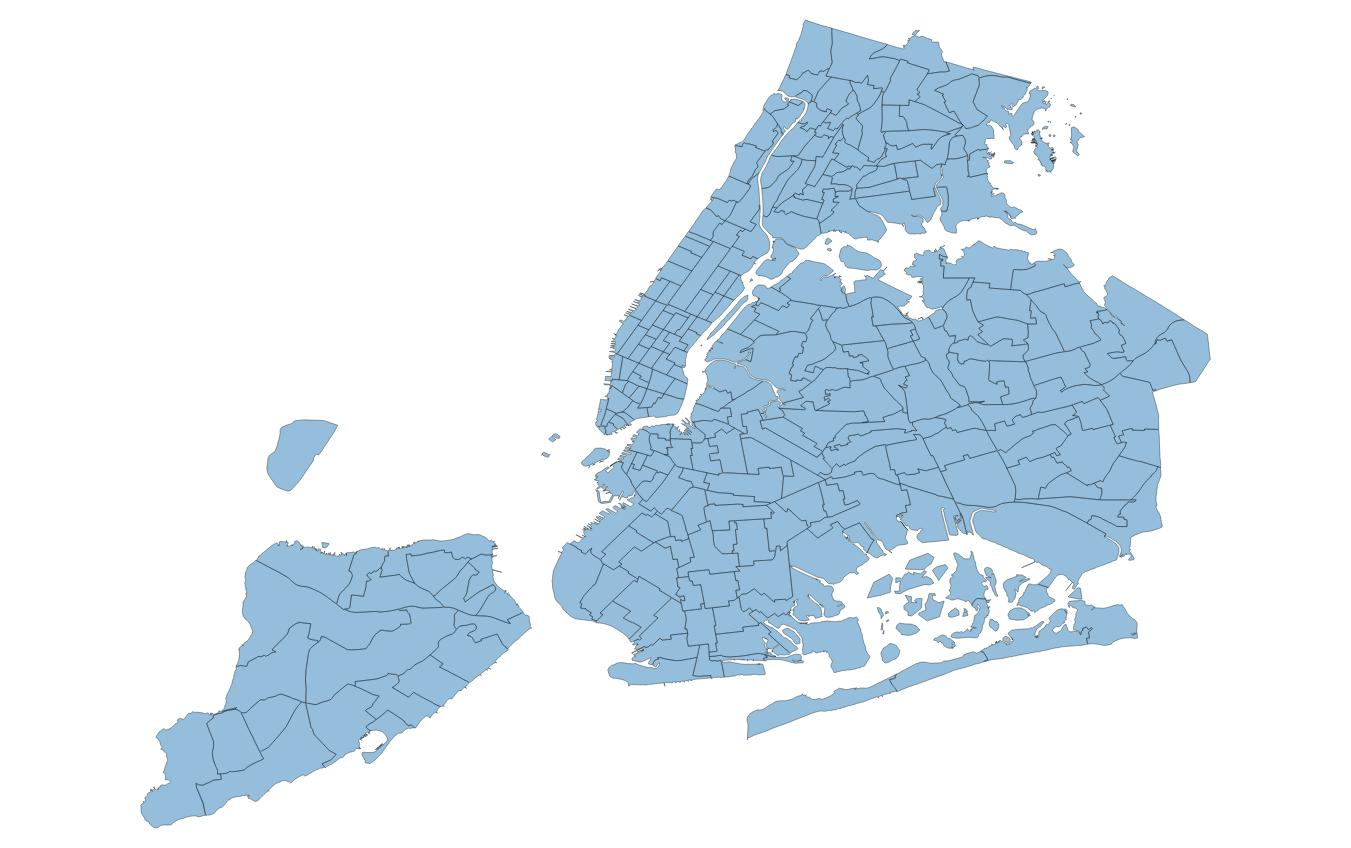
\includegraphics[height=1.4in]{../latex/images/taxi_zones_shape}
      \caption{Shape}
  \end{subfigure}%
  ~ 
  \begin{subfigure}[t]{0.45\textwidth}
      \centering
      \label{fig:zones_raster}
      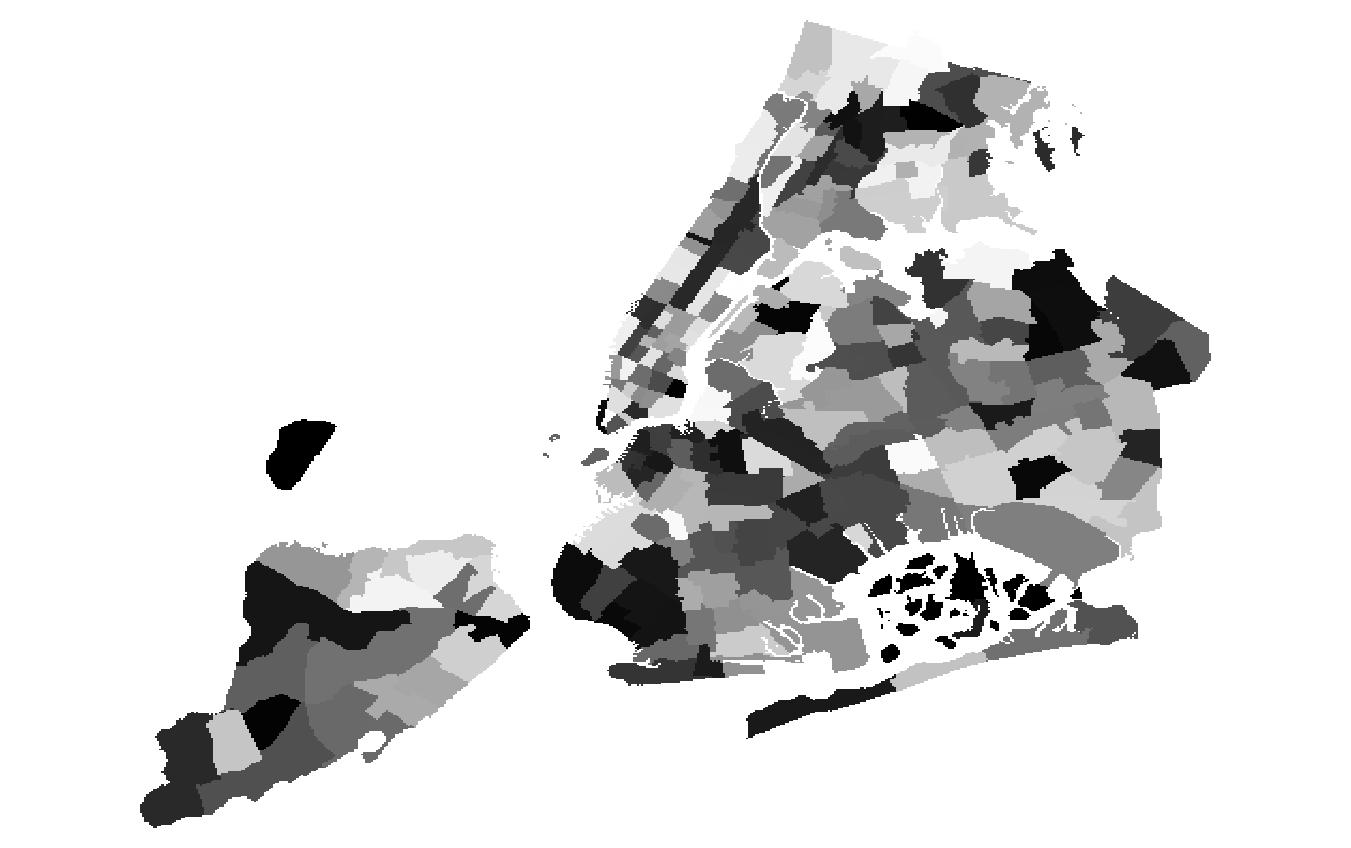
\includegraphics[height=1.4in]{../latex/images/taxi_zones_raster}
      \caption{Raster}
  \end{subfigure}
  \caption{NYC Taxi zones file formats}
    \end{figure}
\end{itemize}

\end{block}

\end{frame}

\begin{frame}

\begin{figure}
    \begin{subfigure}[t]{0.8\textwidth}
        \centering
        \label{fig:zones_both}
        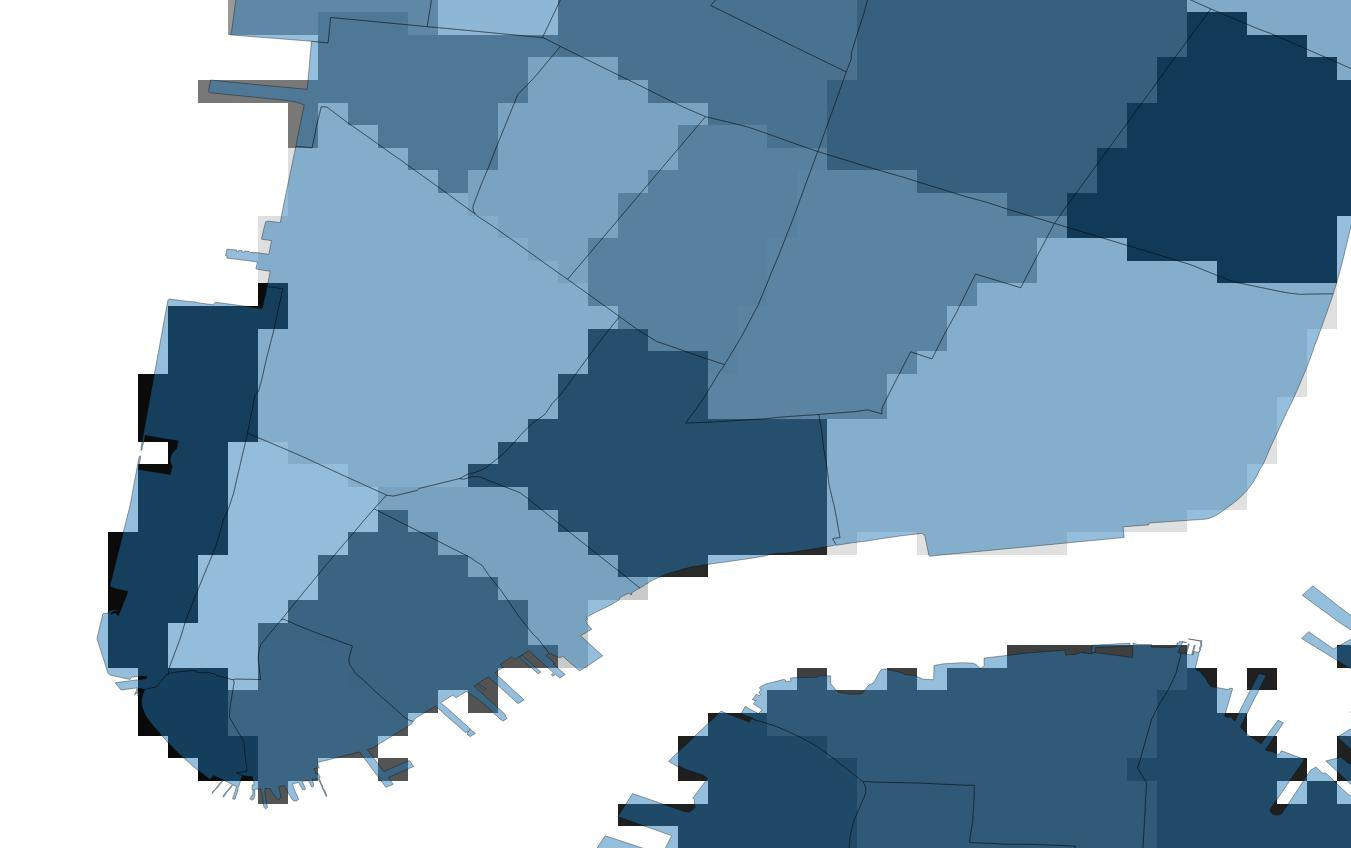
\includegraphics[width=0.5\textwidth]{../latex/images/both}
        \caption{Both}
    \end{subfigure}
    \caption{NYC Taxi zones file formats}
\end{figure}

\end{frame}

\begin{frame}

\begin{block}{Cleaning the data: Crime}

\begin{itemize}
\item
  Dates needed to be cleaned. (\textbf{24:00:00 vs 00:00:00})
\item
  Meaningful interpretations of other dates could not be made for
  certain records and these records had to be filtered for example:

  \begin{itemize}
  \tightlist
  \item
    1016 \(\rightarrow\) 2016.
  \item
    1026 \(\rightarrow\) dropped.
  \end{itemize}
\item
  The most challenging factor here was that I had a lot of missing
  values for some columns so I needed to setup a schema that accepted
  this fact.
\end{itemize}

\end{block}

\begin{block}{Cleaning the data: Weather}

\begin{itemize}
\tightlist
\item
  Weather data was the most decent.
\item
  I basically just checked that the data was clean.
\item
  The only major issue was to figure out a way to assign weather data to
  the taxis.
\end{itemize}

\end{block}

\end{frame}

\begin{frame}

\begin{block}{Joining the data}

\begin{itemize}
\item
  In the cleaning process I assigned taxi zones for taxi pickup and
  drop-off locations.
\item
  So I repeated this process but this time instead of assigning zones I
  assigned a station (JFK, La Guardia, Central Park) by computing the
  min distance from the pickup locations (long/lat) to the weather
  station.
\item
  I had another problem here because I did not have (long/lat) for the
  recent data.
\item
  So, I estimated the centroids on the pick-up zones and then computed
  the min distance to the weather stations.
\item
  Finally taxis were joined to crime by using time periods of one hour.
\end{itemize}

\end{block}

\end{frame}

\begin{frame}{%
\protect\hypertarget{goodness}{%
Goodness}}

\begin{block}{Consistent data}

\begin{itemize}
\tightlist
\item
  One of the main concerns was the consistency of the data through time
  and among the different sources, so I made a lot of effort to keep all
  variables, even the ones I ended up not using.
\end{itemize}

\end{block}

\begin{block}{Empirical observations not causality}

\begin{itemize}
\tightlist
\item
  Up to now I am not trying to explain causality so the observations
  should be interpreted as empirical correlations and raw insight
  obtained from a very long cleaning data phase
\end{itemize}

\end{block}

\end{frame}

\begin{frame}{%
\protect\hypertarget{results}{%
Results}}

\begin{itemize}
\tightlist
\item
  Opposite colors support the hypothesis.

  \begin{figure}
  \label{fig:zones}
    \centering
    \begin{subfigure}[t]{0.45\textwidth}
        \centering
        \label{fig:zones_shape}
        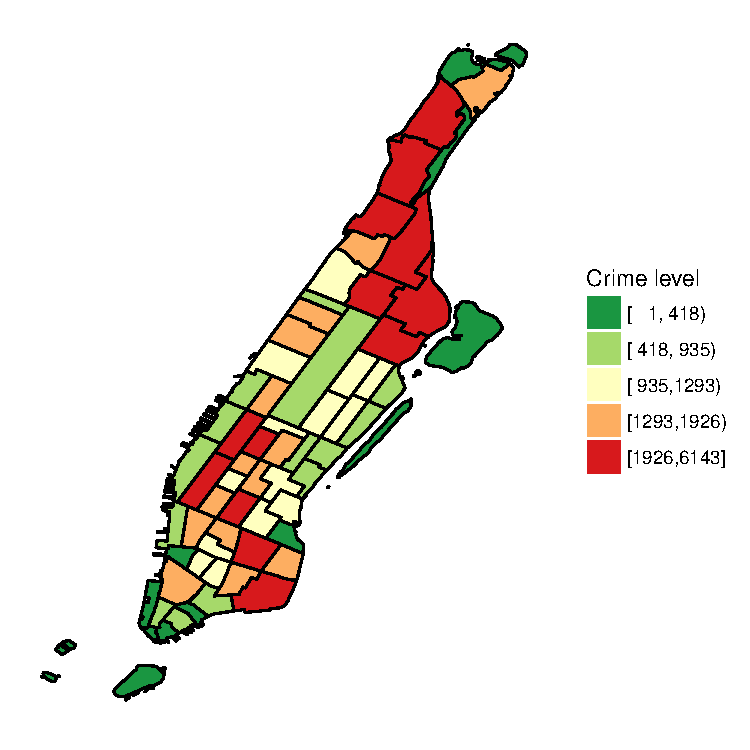
\includegraphics[width=1\textwidth]{../img/crimes_per_zone_2015_Manhattan}
        \caption{Crimes in Manhattan}
    \end{subfigure}%
    ~ 
    \begin{subfigure}[t]{0.45\textwidth}
        \centering
        \label{fig:zones_raster}
        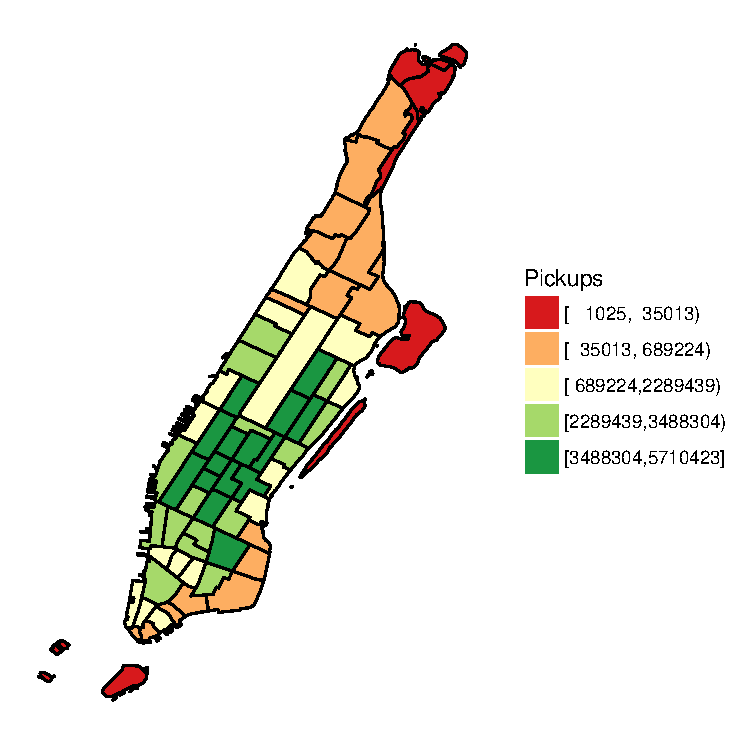
\includegraphics[width=1\textwidth]{../img/taxis_2015_Manhattan}
        \caption{Pickups in Manhattan}
    \end{subfigure}
    \caption{Crime and Pickups in Manhattan, 2015}
  \end{figure}
\end{itemize}

\end{frame}

\begin{frame}

\begin{figure}
  \label{fig:zones}
    \centering
    \begin{subfigure}[t]{0.45\textwidth}
        \centering
        \label{fig:zones_shape}
        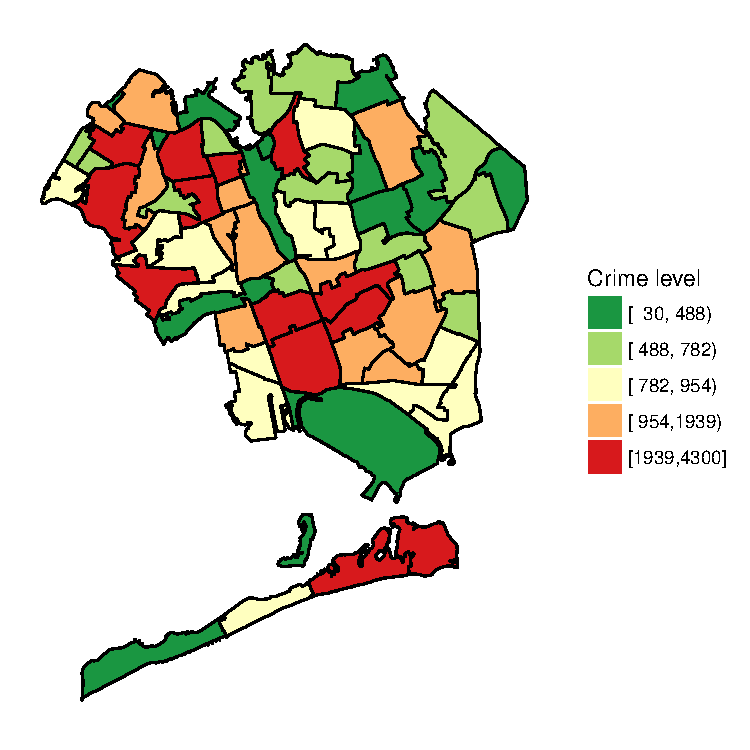
\includegraphics[width=1\textwidth]{../img/crimes_per_zone_2015_Queens}
        \caption{Crimes in Queens}
    \end{subfigure}%
    ~ 
    \begin{subfigure}[t]{0.45\textwidth}
        \centering
        \label{fig:zones_raster}
        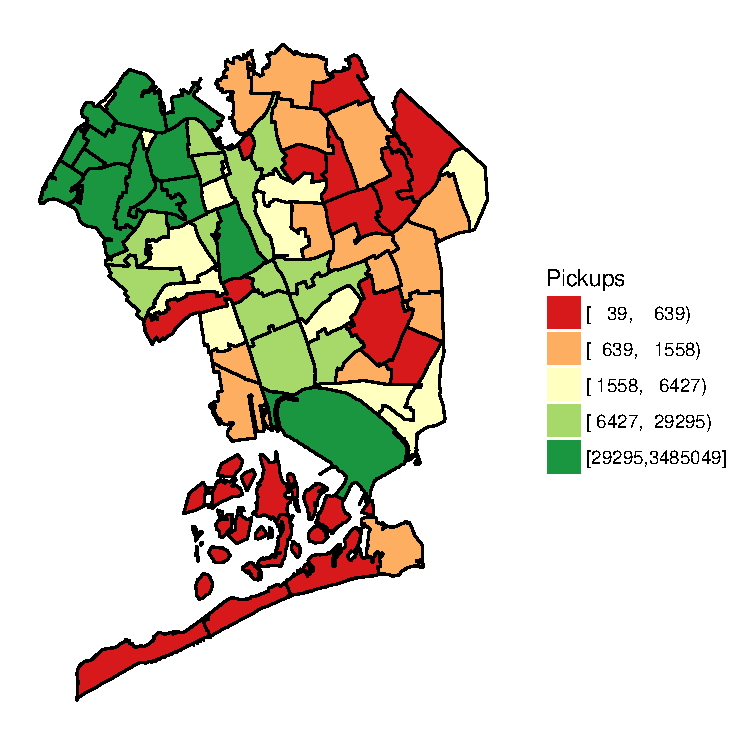
\includegraphics[width=1\textwidth]{../img/taxis_2015_Queens}
        \caption{Pickups in Queens}
    \end{subfigure}
    \caption{Crime and Pickups in Queens, 2015}
  \end{figure}

\end{frame}

\begin{frame}

\begin{block}{Crimes and taxis}

\begin{figure} 
\centering
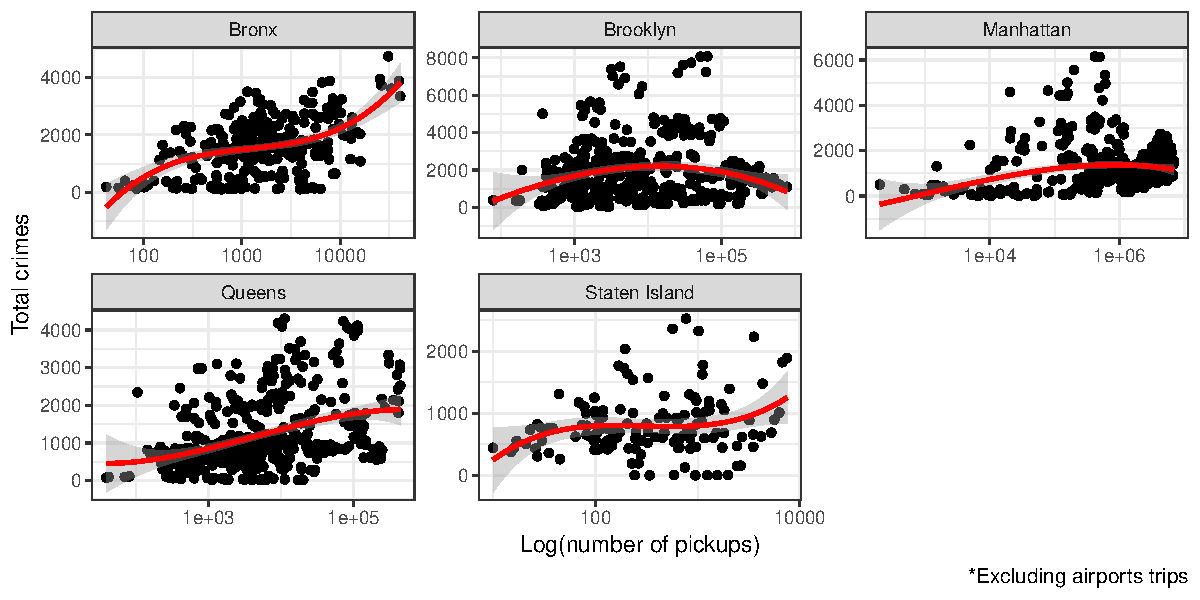
\includegraphics[width=1\textwidth]{../img/scatter_crimes_taxis_pres.pdf}
\caption{Crimes and pickups per zone}
\end{figure}

\end{block}

\end{frame}

\begin{frame}

\begin{block}{Results when considering Rain}

\begin{figure} 
\centering
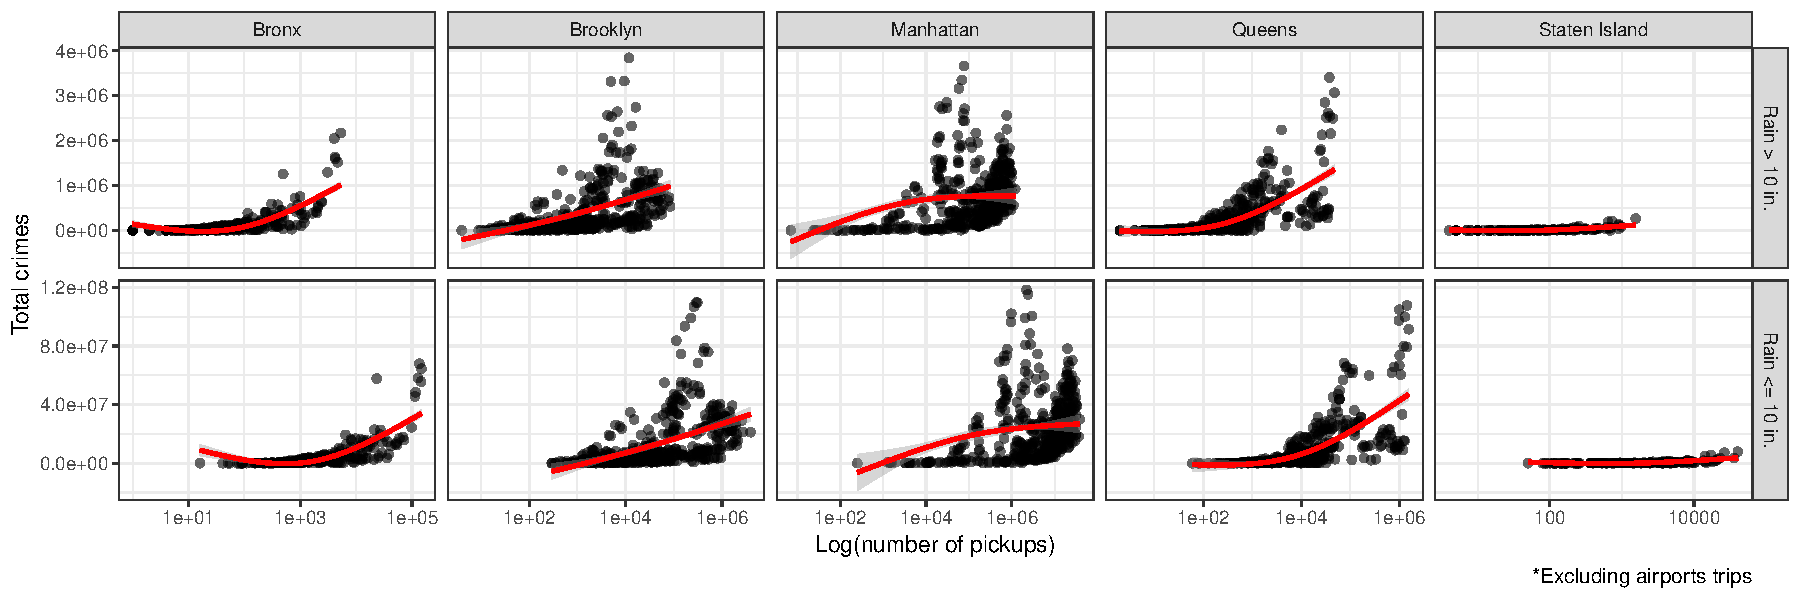
\includegraphics[width=1\textwidth]{../img/scatter_crimes_taxis_rain.pdf}
\caption{Crimes and hourly pickups per zone in rain}
\end{figure}

\end{block}

\end{frame}

\begin{frame}{%
\protect\hypertarget{summary}{%
Summary}}

\begin{itemize}
\item
  I collected NYC taxi trip data, NYC crime data and weather data from
  Central Park, JFK and LaGuardia and I was able to join everything at a
  very granular level.
\item
  I found evidence that suggests that the hypothesis might be true,
  places that have higher levels of crime showed evidence of having a
  higher number of pickups, especially when taking rain into account.
\end{itemize}

\end{frame}

\begin{frame}{%
\protect\hypertarget{references}{%
References}}

\begin{thebibliography}{1}

\bibitem{Bendler14}
J.~Bendler, T.~Brandt, S.~Wagner, and D.~Neumann.
\newblock Investigating crime-to-twitter relationships in urban environments -
  facilitating a virtual neighborhood watch.
\newblock In M.~Avital, J.~M. Leimeister, and U.~Schultze, editors, {\em ECIS},
  2014.

\bibitem{Wang16}
H.~Wang, D.~Kifer, C.~Graif, and Z.~Li.
\newblock Crime rate inference with big data.
\newblock In {\em Proceedings of the 22Nd ACM SIGKDD International Conference
  on Knowledge Discovery and Data Mining}, KDD '16, pages 635--644, New York,
  NY, USA, 2016. ACM.

\bibitem{Traunmueller14}
M.~Traunmueller, G.~Quattrone, and L.~Capra.
\newblock {\em Mining Mobile Phone Data to Investigate Urban Crime Theories at
  Scale}, pages 396--411.
\newblock Springer International Publishing, Cham, 2014.
\end{thebibliography}

\end{frame}

\begin{frame}

\begin{thebibliography}{1}
\bibitem{OUAC}
A.~Bogomolov, B.~Lepri, J.~Staiano, N.~Oliver, F.~Pianesi, and A.~Pentland.
\newblock Once upon a crime: Towards crime prediction from demographics and
  mobile data, Sep 2014.

\bibitem{Chainey}
S.~Chainey, L.~Tompson, and S.~Uhlig.
\newblock {The Utility of Hotspot Mapping for Predicting Spatial Patterns of
  Crime}.
\newblock {\em Security Journal}, 21(1-2):4--28, Feb 2008.

\bibitem{visCrime}
T.~Nakaya and K.~Yano.
\newblock Visualising crime clusters in a space-time cube: An exploratory
  data-analysis approach using space-time kernel density estimation and scan
  statistics.
\newblock {\em Transactions in GIS}, 14(3):223--239, 2010.
\end{thebibliography}

\end{frame}

\end{document}
